\documentclass[11pt,a4paper]{article}
\usepackage{fullpage}
\usepackage{graphicx}
\usepackage{siunitx}
\usepackage{amsmath}
\usepackage{booktabs}
\usepackage{bm}
\usepackage[hidelinks]{hyperref}
\usepackage[noabbrev, capitalise]{cleveref}

\sisetup{input-digits=0123456789\pi}

\title{Consideration of objects between a camera and the target for infrared measurements}

\author{Andrew Hurlbatt}

\date{\today}

\renewcommand{\abstractname}{\vspace{-\baselineskip}}

\begin{document}
	
	\maketitle
	
	\begin{abstract}
		In making infrared measurements, it is usually the case that objects, including air, exist between the camera and the target that can affect the infrared radiation between the two. In addition, all objects reflect some amount of radiation from the environment. A method is detailed here of using summary properties of the objects involved to estimate the actual radiance emitted toward the detector by the target. Self-emission, transmittances, and reflectances of all objects are considered, also allowing for separation of diffuse and specular reflections, as well as reflections between objects.
	\end{abstract}

\section{Object Properties}

When using infrared imaging to measure object temperatures, there are often objects along the imaging path that may alter the radiation through absorption, reflection, or addition of their own emission. These should all be taken into account as far as practicable when using a measured radiance to estimate that of a target. Starting with an isolated object, that object may be emitting radiation due to its temperature. If the object is a black body, the emitted radiation is defined by the Stefan-Boltzmann Law (\cref{eq:sb_law}) to give the radiance of a black body ($ L^\circ $) at a given temperature in Kelvin ($ T $), depending on the Stefan-Boltzmann constant ($ \sigma $).

\begin{equation}\label{eq:sb_law}
	L^\circ = \frac{\sigma}{\pi} T^4
\end{equation}

As objects are unlikely to be perfect black bodies, the actual radiance will be lower than that calculated by \cref{eq:sb_law}, where the reduction factor $ \epsilon \le 1 $ is the emittance of the object (or a particular surface of an object).

The effect of the object on incoming radiation also needs to be considered. In general, there are three possible outcomes for radiation that is incident on the surface of the object: absorption, reflection, or transmission. The amount of absorbed, reflected, and transmitted radiation relative to the power of the incoming radiation is determined by the absorptance $ \alpha $, reflectance $ \rho $, and transmittance $ \tau $.%
\footnote{There is some ambiguity in the literature as to the exact names of the coefficients, in particular between \emph{emittance} and \emph{emissivity}. In this work the \emph{-tance} suffix will be used, and hopefully it is clear from their definitions here that they are dimensionless ratios, and not absolute quantities.} %
The absorptance $ \alpha $ is equated to the emittance $ \epsilon $ by Kirchoff's law of thermal radiation. As absorption, reflection, and transmission are the only possibilities, and all of the incoming radiation must be accounted for, it stands that the respective coefficients must sum to unity as in \cref{eq:unity}, where Kirchoff's law is used to replace $ \alpha $ with $ \epsilon $.

\begin{equation}\label{eq:unity}
	\epsilon + \rho + \tau = 1
\end{equation}

For radiation that is reflected, there is an angular dependence on the distribution of outgoing radiation. In the idealised, microscopic, case the direction of the incoming radiation is mirrored in the surface normal to give the direction of the outgoing radiation - specular reflection. From the macroscopic perspective, a only a perfectly smooth surface leads to true specular reflection. In the other extreme case, outgoing radiation is scattered over the \SI{2\pi}{\steradian} of the hemisphere - diffuse reflection. Various models exists for how to consider the angular distribution of reflections from real surfaces; in this work, surfaces will be modelled as reflecting a combination of these two extreme cases. The reflectance $ \rho $ corresponds to the total ratio of radiation that is reflected, and the amount of this that is reflected diffusely is given by the diffuse fraction $ D $. Therefore the relative amount of  incoming radiation that is reflected diffusely is found using $ D\rho $. Correspondingly, the relative amount of specularly reflected radiation is given by $ \left(1 - D\right)\rho $.

If an object has a non-zero specular reflectance, then it is important to consider from which direction radiation is reflected. If the reflecting surface is perpendicular to the line between the detector and the target (the optical axis), then radiation coming from the direction of the target will be reflected back toward the target, and similarly in the direction of the detector. If it is not aligned, then radiation from the surrounding environment - background radiation $ L_B $ - will be reflected into the path between the target and the detector. To define if an object is aligned with the optical axis, it is given a parameter $ g \in \left\{0,1\right\}$, where a zero indicates that the object is not aligned, and that specular reflections will be from the background of that object $ L_{B,n} $. As an approximation, diffusely reflected radiation from a directed source, such as radiation from the target object scattered from an imperfect window surface, is considered lost, due to the vanishingly small proportion of this that would remain within the axis of the detector.

There is an additional complicating factor, in that the detector in use will not have a perfect spectral response, and properties of objects are likely to depend on wavelength. In theory, all of the quantities so far mentioned should be indicated as depending on wavelength $ \lambda $, and the final equations integrated over $ \lambda $. In practice, object properties can be approximated by single values, either pre-integrated if the spectral behaviour of both the object and the detector are known, or measured using the same detector that will be used for the final application. As these considerations are unique for particular use cases, properties here will be considered as single values, with spectral properties already considered. Conversion between temperature and \emph{apparent} radiance also depends on the specific detector or camera in use. In this work, radiance values $ L^\circ_n $ represent that of a black body at the same temperature as object $ n $, as measured by a specific detector. True radiance values can be obtained using properties of the detector, such as the aperture size, but that is beyond the scope of this work, and also relies upon assuming that the distance between the detector and the target object is large enough such that small angle approximations can be used.

An list of the properties that need to be considered for objects is given in \cref{tab:properties}. An example arrangement of objects is given in \cref{fig:scheme}. This figure also shows the quantities $ F_n $ and $ B_n $, which correspond to the radiation that is travelling forwards - toward the detector - and backwards - toward the target object - between objects $ n $ and $ n+1 $. Background radiation incident on each object is also shown, as well as $ L_M $, the apparent radiance measured by the detector.

\begin{table}
	\centering
	\begin{tabular}{r|p{100mm}}
		\toprule
		Property& Description \\
		\midrule
		$ T_n $& Temperature [\si{\kelvin}]  \\
		$ L^\circ_n $& Apparent radiance of a black body at the temperature $ T_n $, as measured by a specific detector \si{\watt\per\steradian\per\square\metre} \\
		$\epsilon_n$& Emittance \\
		$\tau_n$& Transmittance \\
		$ \rho_n $& Reflectance \\
		$ D_n $& Diffuse reflection fraction\\
		$ g_n $& Axis alignment flag $ \in \left\{0,1\right\} $\\
		$ L_{B,n} $& Background radiation incident on the object\\
		\bottomrule
	\end{tabular}
\caption{The summary properties of object $ n $ within the path between the detector and the target object.}
\label{tab:properties}
\end{table}

\begin{figure}
	\centering
	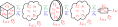
\includegraphics[width=\textwidth]{./infrobjects_scheme.pdf}
	\caption{An example system with a window between the camera and the target, showing the atmosphere between each object should also be considered.}
	\label{fig:scheme}
\end{figure}

\section{Finding Transported Radiation}

Working backwards from the detector in \cref{fig:scheme}, the forward radiation in the first gap, $ F_0 $, should be equal to the measured radiance $ L_M $, minus any that is reflected away if $ \rho_0 $ is not zero. The backward radiation $ B_0 $ may contain the fraction of $ F_0 $ that is reflected from the detector, as well as reflections from the background $ L_{B,0} $ and self emission from the detector $ \epsilon_0 L^\circ_0 $.

Taking a step toward the target object, to object $ n=1 $, the previously mentioned forward radiation, $ F_0 $, must be the result of the interaction of object $ n=1 $ with the ``previous'' forward radiation $ F_1 $ and the incoming backward radiation $ B_0 $, as well as emission from the object itself and reflections from the background. The backward radiation $ B_1 $ will also result from these interactions. The contributions to these quantities are given in \cref{eq:F0,eq:B0} and explained below.
\begin{align}
	F_0 &= \tau_1 F_1 + g_1 \left(1 - D_1\right) \rho_1 B_0 + \epsilon_1 L^\circ_1 + D_1 \rho_1 L_{B,1} + \left(1 - g_1\right)\left(1 - D_1\right) \rho_1 L_{B,1} \label{eq:F0}\\
	B_1 &= \tau_1 B_0 + g_1 \left(1 - D_1\right) \rho_1 F_1 + \epsilon_1 L^\circ_1 + D_1 \rho_1 L_{B,1} + \left(1 - g_1\right)\left(1 - D_1\right) \rho_1 L_{B,1} \label{eq:B0}
\end{align}

In \cref{eq:F0,eq:B0}, the contributions are:
\begin{itemize}
	\item $ \tau_1 F_1 $ --- transmission of $ F_1 $ through the object
	\item $ \tau_1 B_0 $ --- transmission of $ B_0 $ through the object
	\item $ g_1 \left(1 - D_1\right) \rho_1 B_0 $ --- (possible) specular reflection of $ B_0 $ from the object
	\item $ g_1 \left(1 - D_1\right) \rho_1 F_1 $ --- (possible) specular reflection of $ F_1 $ from the object
	\item $ \epsilon_1 L^\circ_1 $ --- self-emission of the object
	\item $ D_1 \rho_1 L_{B,1} $ --- diffuse reflection of background radiation
	\item $ \left(1 - g_1\right)\left(1 - D_1\right) \rho_1 L_{B,1} $ --- (possible) specular reflection of background radiation
\end{itemize}

As \cref{eq:F0,eq:B0} consider all possible interactions of incoming radiation with object $ n=1 $, they can be applied to any object $ n $ to find relationships between incoming $ F_n $ and $ B_{n-1} $, and the outgoing $ F_{n-1} $ and $ B_n $ that depend on the properties of object $ n $.

After rearrangement to solve for $ F_n $, \cref{eq:F0} becomes:
\begin{equation}\label{eq:Fn}
	F_n = \frac{1}{\tau_n} F_{n-1} - g_n \left(1 - D_n\right) \frac{\rho_n}{\tau_n} B_{n-1} - \frac{\epsilon_n}{\tau_n} L^\circ_n - \left[D_n + \left(1 - g_n\right)\left(1 - D_n\right)\right] \frac{\rho_n}{\tau_n} L_{B,n}
\end{equation}

Through simple substitution \cref{eq:B0} becomes:
\begin{equation}\label{eq:Bn_1}
	B_n = \tau_n B_{n-1} + g_n \left(1 - D_n\right) \rho_n F_n + \epsilon_n L^\circ_n + \left[D_n + \left(1 - g_n\right)\left(1 - D_n\right)\right] \rho_n L_{B,n}
\end{equation}

As will be seen later, it is useful to have the equations for both $ F_n $ and $ B_n $ to be in terms only of $ F_{n-1} $ and $ B_{n-1} $ and the properties of object $ n $. To achieve this, \cref{eq:Fn} is substituted into \cref{eq:Bn_1} to obtain \cref{eq:Bn_2}. In this derivation, the property of $ g_n \in \left\{0,1\right\} $ is used to conclude that $ g_n \left(1 - g_n\right) = 0 $ and that $ g_n^2 = g_n $. The derivation is detailed in \cref{sec:Bn}.
\begin{equation}\label{eq:Bn_2}
\begin{split}
	B_n = & 
		\left[ \tau_n - g_n \left(1 - D_n\right)^2 \frac{\rho_n^2}{\tau_n} \right] B_{n-1}
		+ g_n \left(1 - D_n\right) \frac{\rho_n}{\tau_n} F_{n-1} \\&
		+ \left[ 1 - g_n \left(1 - D_n\right) \frac{\rho_n}{\tau_n} \right] \epsilon_n L^\circ_n
		+ \left[1 - g_n \left( 1 - D_n \right) \left(1 + D_n \frac{\rho_n}{\tau_n}\right) \right] \rho_n L_{B,n}
\end{split}
\end{equation}

\section{Matrix Expressions}

The \cref{eq:Fn,eq:Bn_2} comprise a pair of coupled, recursive linear equations. To find the next $ F_n $ and $ B_n $, one needs the previous $ F_{n-1} $ and $ B_{n-1} $ and the properties of object $ n $. As the equations are linear, they can be collected into the following matrices.

\begin{align*}
	\bm{X}_n &=
		\begin{bmatrix}
			F_n \\ B_n
		\end{bmatrix}
	&
	\bm{A}_n &=
		\begin{bmatrix}
			\frac{1}{\tau_n} & - g_n \left(1 - D_n\right) \frac{\rho_n}{\tau_n} \\
			g_n \left(1 - D_n\right) \frac{\rho_n}{\tau_n} & \tau_n - g_n \left(1 - D_n\right)^2 \frac{\rho_n^2}{\tau_n} \\
		\end{bmatrix}
\end{align*}
\begin{equation*}
	\bm{b}_n = 
		\begin{bmatrix}
			- \frac{\epsilon_n}{\tau_n} L^\circ_n - \left[D_n + \left(1 - g_n\right)\left(1 - D_n\right)\right] \frac{\rho_n}{\tau_n} L_{B,n}\\[5pt]
			\left[1 - g_n \left(1 - D_n\right) \frac{\rho_n}{\tau_n}\right] \epsilon_n L^\circ_n + \left[1 - g_n \left( 1 - D_n \right) \left(1 + D_n \frac{\rho_n}{\tau_n}\right) \right] \rho_n L_{B,n}
		\end{bmatrix}
\end{equation*}

In the case where $ g_n = 0 $, $ \bm{A}_n $ and $ \bm{b}_n $ simplify to:
\begin{align*}
	\bm{A}_n &=
		\begin{bmatrix}
			\frac{1}{\tau_n} & 0 \\
			0 & \tau_n \\
		\end{bmatrix}
	&
	\bm{b}_n &= 
	\begin{bmatrix}
		-\frac{1}{\tau_n}\\[5pt]
		1
	\end{bmatrix} \left(\epsilon_n L^\circ_n + \rho_n L_{B,n}\right)
\end{align*}

In the case where $ g_n = 1 $, $ \bm{A}_n $ and $ \bm{b}_n $ simplify to:
\begin{align*}
	\bm{A}_n &=
		\begin{bmatrix}
			\frac{1}{\tau_n} & - \left(1 - D_n\right) \frac{\rho_n}{\tau_n} \\
			\left(1 - D_n\right) \frac{\rho_n}{\tau_n} & \tau_n - \left(1 - D_n\right)^2 \frac{\rho_n^2}{\tau_n} \\
		\end{bmatrix}
	&
	\bm{b}_n &= 
		\begin{bmatrix}
			-\frac{1}{\tau_n} \\[5pt]
			1 - \left(1 - D_n\right) \frac{\rho_n}{\tau_n}
		\end{bmatrix} \left(\epsilon_n L^\circ_n + D_n \rho_n L_{B,n}\right)
\end{align*}

From these matrices, \cref{eq:Fn,eq:Bn_2} can be collected into a single matrix equation given as \cref{eq:matrix_1}.
\begin{equation}\label{eq:matrix_1}
	\bm{X}_n = \bm{A}_n \bm{X}_{n-1} + \bm{b}_n
\end{equation}

To solve this equation for a system of $ N $ objects, plus a target object $ T $, one needs to define an initial value $ \bm{X}_0 $ and enable the calculation of an arbitrary $ \bm{X}_N $ given the properties of objects $ n = 1 \dots N $. Successive applications of \cref{eq:matrix_1} result in repeated multiplications and additions, summarized in \cref{eq:matrix_2}. In this and following expressions, ``Big-Pi'' notation is used to mean matrix multiplication, with subsequent terms being ordered left to right.
\begin{equation}\label{eq:matrix_2}
	\bm{X}_n = \left(\prod_{i=0}^{n-1} \bm{A}_{n-i}\right) \bm{X}_0 + \sum_{i=1}^{n-1} \left( \prod_{j=0}^{n-i-1} \bm{A}_{n-j} \right) \bm{b}_i + \bm{b}_n
\end{equation}

By isolating the two constant terms, they can be taken out of the expression and evaluated individually to give a single, non-recursive, expression for $ \bm{X}_N $ in \cref{eq:X_N}.

\begin{align*}
		\bm{E}_n &= \prod_{i=0}^{n-1} \bm{A}_{n-i} &
		\bm{C}_n &= \sum_{i=1}^{n-1} \left( \prod_{j=0}^{n-i-1} \bm{A}_{n-j} \right) \bm{b}_i + \bm{b}_n
\end{align*}

\begin{equation}\label{eq:X_N}
	\bm{X}_{N} = \bm{E}_N \bm{X}_0 + \bm{C}_N
\end{equation}

The value of $ \bm{X}_N = \left[F_N \enspace B_N\right]^T $, corresponding to $ F_3 $ and $ B_3 $ in \cref{fig:scheme}, do not immediately give the properties of the target object, which also has its own emittance and reflectance etc. Typically, it is also assumed that the target object has transmittance $ \tau_T = 0 $, so that $ \rho_T = 1 - \epsilon_T $. Using this, \cref{eq:F0} can be repurposed to give \cref{eq:FN}, an expression for $ F_N $ using the properties of the target object, including the desired quantity $ L^\circ_T $. Rearranging this gives \cref{eq:MT_1}, an expression for $ L^\circ_T $.
\begin{equation}\label{eq:FN}
	F_N = g_T \left(1 - D_T\right) \rho_T B_N + \epsilon_T L^\circ_T + D_T \rho_T L_{B,T} + \left(1 - g_T\right)\left(1 - D_T\right) \rho_T L_{B,T}
\end{equation}
\begin{equation}\label{eq:MT_1}
	L^\circ_T = \frac{1}{\epsilon_T} F_N - g_T \left(1 - D_T\right) \frac{\rho_T}{\epsilon_T} B_N - \left[D_T + \left(1 - g_T\right)\left(1 - D_T\right) \right] \frac{\rho_T}{\epsilon_T} L_{B,T}
\end{equation}

To find $ L^\circ_T $ directly from $ \bm{X}_N $, two new variables are defined that can be used with the matrix formulation of \cref{eq:X_N}. Combining these expressions results in \cref{eq:MT_2}.
\begin{align*}
	\bm{H}_T &=
	\begin{bmatrix}
		\frac{1}{\epsilon_T} & - g_T \left(1 - D_T\right) \frac{\rho_T}{\epsilon_T}
	\end{bmatrix}
&
K_T &= \left[D_T + \left(1 - g_T\right)\left(1 - D_T\right) \right] \frac{\rho_T}{\epsilon_T} L_{B,T}
\end{align*}
\begin{equation}\label{eq:MT_2}
	L^\circ_T = \bm{H}_T \left( \bm{E}_N \bm{X}_0 + \bm{C}_N \right) - K_T
\end{equation}

To find values for $ \bm{X}_0 $, some assumptions need to be made about the detector. Firstly, the measured radiance $ L_M $ is assumed to correspond to the incoming radiation $ F_0 $, without any modifications, all of which should be accounted for during the detector calibration process. Secondly, the reflection of background radiation from the detector toward the target is assumed negligible, such that only the temperature and radiance of the detector itself needs to be considered. Thus $ \bm{X}_0 = \left[ L_M \enspace L^\circ_0 \right]^T $.

The coefficients of the linear expression in \cref{eq:MT_2} are independent of the measured radiance, and therefore only need to be calculated once for each system, which can improve efficiency.

\appendix
\numberwithin{equation}{section}

\section{Derivation of $ B_n $}\label{sec:Bn}

\begin{align}
\begin{split}
	B_n = & \tau_n B_{n-1} + g_n \left(1 - D_n\right) \rho_n F_n + \epsilon_n L^\circ_n + \left[D_n + \left(1 - g_n\right)\left(1 - D_n\right)\right] \rho_n L_{B,n}
\end{split}\\
\begin{split}
	B_n = & \tau_n B_{n-1} + \epsilon_n L^\circ_n + \left[D_n + \left(1 - g_n\right)\left(1 - D_n\right)\right] \rho_n L_{B,n} + g_n \left(1 - D_n\right) \rho_n \times \\ &\left(\frac{1}{\tau_n} F_{n-1} - g_n \left(1 - D_n\right) \frac{\rho_n}{\tau_n} B_{n-1} - \frac{\epsilon_n}{\tau_n} L^\circ_n - \left[D_n + \left(1 - g_n\right)\left(1 - D_n\right)\right] \frac{\rho_n}{\tau_n} L_{B,n}\right)
\end{split}\\
\begin{split}
	B_n = & 
		\tau_n B_{n-1}
		+ \epsilon_n L^\circ_n
		+ \left[D_n + \left(1 - g_n\right)\left(1 - D_n\right)\right] \rho_n L_{B,n} \\&
		+ g_n \left(1 - D_n\right) \rho_n \frac{1}{\tau_n} F_{n-1} \\&
		- g_n \left(1 - D_n\right) \rho_n g_n \left(1 - D_n\right) \frac{\rho_n}{\tau_n} B_{n-1} \\&
		- g_n \left(1 - D_n\right) \rho_n \frac{\epsilon_n}{\tau_n} L^\circ_n \\&
		- g_n \left(1 - D_n\right) \rho_n \left[D_n + \left(1 - g_n\right)\left(1 - D_n\right)\right] \frac{\rho_n}{\tau_n} L_{B,n}
\end{split}\\
\begin{split}
	B_n = & 
		\tau_n B_{n-1}
		+ \epsilon_n L^\circ_n
		+ \left[D_n + \left(1 - g_n\right)\left(1 - D_n\right)\right] \rho_n L_{B,n} \\&
		+ g_n \left(1 - D_n\right) \frac{\rho_n}{\tau_n} F_{n-1} \\&
		- g_n^2 \left(1 - D_n\right)^2 \frac{\rho_n^2}{\tau_n} B_{n-1} \\&
		- g_n \left(1 - D_n\right) \frac{\epsilon_n \rho_n}{\tau_n} L^\circ_n \\&
		- \left[g_n D_n \left(1 - D_n\right) + g_n \left(1 - g_n\right) \left(1 - D_n\right)^2 \right] \frac{\rho_n^2}{\tau_n} L_{B,n}
\end{split}\\
\begin{split}
	B_n = & 
		\tau_n B_{n-1}
		- g_n \left(1 - D_n\right)^2 \frac{\rho_n^2}{\tau_n} B_{n-1} \\&
		+ g_n \left(1 - D_n\right) \frac{\rho_n}{\tau_n} F_{n-1} \\&
		+ \epsilon_n L^\circ_n
		- g_n \left(1 - D_n\right) \frac{\epsilon_n \rho_n}{\tau_n} L^\circ_n \\&
		+ \left[D_n + \left(1 - g_n\right)\left(1 - D_n\right)\right] \rho_n L_{B,n}
		- g_n D_n \left(1 - D_n\right) \frac{\rho_n}{\tau_n} \rho_n L_{B,n}
\end{split}\\
\begin{split}
	B_n = & 
		\tau_n B_{n-1}
		- g_n \left(1 - D_n\right)^2 \frac{\rho_n^2}{\tau_n} B_{n-1} \\&
		+ g_n \left(1 - D_n\right) \frac{\rho_n}{\tau_n} F_{n-1} \\&
		+ \left[1 - g_n \left(1 - D_n\right) \frac{\rho_n}{\tau_n}\right] \epsilon_n L^\circ_n \\&
		+ \left[1 - g_n \left(1 - D_n\right) \left(1 + D_n \frac{\rho_n}{\tau_n}\right)\right] \rho_n L_{B,n}
\end{split}\\
\begin{split}
	B_n = & 
		\tau_n B_{n-1}
		- \left(1 - D_n\right)^2 \frac{\rho_n^2}{\tau_n} B_{n-1} \\&
		+ \left(1 - D_n\right) \frac{\rho_n}{\tau_n} F_{n-1} \\&
		+ \left[1 - \left(1 - D_n\right) \frac{\rho_n}{\tau_n}\right] \left[\epsilon_n L^\circ_n + D_n \rho_n L_{B,n} \right]
\end{split}
\end{align}

\end{document}